\chapter{DIGITAL MARKETPLACES IN PRACTICE}
\section{Introduction}

In practice, digital marketplace are always unique and have their own product insights that make them successful. This theoretical model is not a prescription for digital marketplaces but rather a framework with which to think about the incentives at play in commodified digital marketplaces. To augment the CDM framework, this paper also explores the practical side of launching and growing digital marketplaces based on my personal research and experience.

\subsection{How the theory fails}.

This theory fails in more ways than one, but here are a few notable departures from practice.

\subsubsection{Market for the service may not exist}

The model assumes that a market for the service already exists, but in practice determining whether the market exists for a service is a large part of reaching product-market fit and cannot be assumed.

\subsubsection{There may not be sufficient supply in the market}

Even if there is a market for a given service, and you could commodify it using technology, there may not be sufficient supply in the market to create a successful commodified digital marketplace. If you wanted to build an on-demand service for disinfecting spaces, there may be sufficient demand and technology, but there may not be enough individuals or companies that want to engage in that service.

\subsection{Real-world challenges of a digital marketplace}

Departing from the CDM model entirely, there are a number of well-documented challenges that digital marketplaces face that are worth noting.

\section{Chicken and the Egg Problem}

Probably the most profound challenge is the chicken and the egg problem. Digital marketplaces are difficult to start because they require two different audiences to be orchestrated together. You need suppliers to attract buyers and buyers to attrack suppliers, but which comes first? Based on research into this topic, here are the top few strategies \citep{whatsNext}.

\subsection{Standalone Mode}

Standalone mode is when the product stands on its own without the marketplace. The product is usually made for one side of the market first, then after attracting users it opens up the marketplace. Users come to the product initially for the standalone mode, and their activity is used to launch a liquid marketplace. An example of this is LinkedIn (a marketplace between workers and companies) starting as a place for people to put their online CV and build their professional network. Similarly, Hire a Student lets students create their work profiles and showcase their work capacity, adding value to students in a market before there are hirers. Another example is OpenTable, which starts off selling reservation software to restaurants in a given market, then opens up the marketplace to diners when the market has sufficient restaurant density.

\subsection{Offering to fill empty seats for suppliers}

Another strategy to solve the chicken and egg problem is to build the market with existing, excess supply. This way, the supply is relatively easy to collect with the promise of incremental revenue.

\subsection{Buyers are sellers}

Another notable way to solve the chicken and egg problem is to make a digital marketplace where buyers are sellers. This way, the marketplace can focus on one target audience and build both sides of the market. This strategy makes it easier to match demand to supply and achieve market liquidity early. An example of this type of digital marketplace is OfferUp \url{https://offerup.com}. 

\section{Hacking Growth}

Another crucial element of any digital marketplace is how they hack growth. A clever growth hack can dramatically lower the cost to acquire new users and kickstart market liquidity.

\subsection{Referral}

One strategy is referral, whereby users are incentivized to refer other users. When I first launched Hire a Student, I created an advocacy program where students earned commission on other student signups. In the first week of launch, I was able to signup several hundred students (nearly 1/3 students at the school) using the referral program.
Over the past few years I have refined the referral program to be a consistent driver of user growth.

\begin{figure}[ht!]
\begin{center}
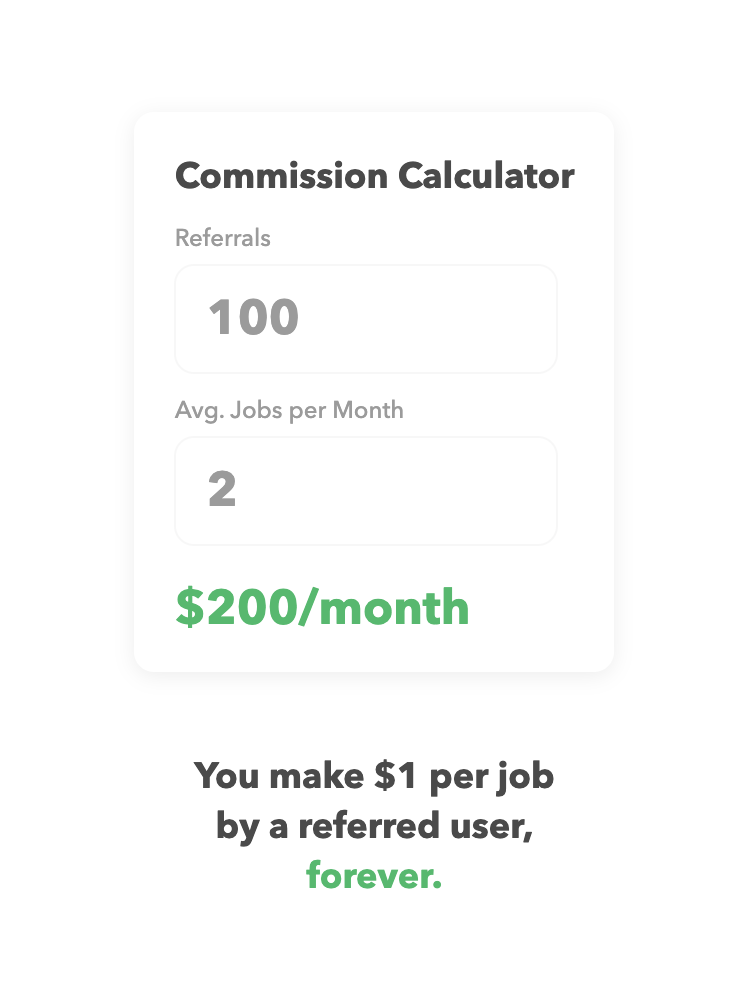
\includegraphics[scale=0.5]{figures/referral.png}
\end{center}
\caption[Example Referral Mechanism]{Hire a Student incentivizes users to refer others}
\label{referral}
\end{figure}

\subsection{Social}

Another strategy is to make the product social, creating no-cost incentives for users to share the app with their friends. Snackpass (\url{https://snackpass.co}), a Yale startup that lets users order food ahead and share rewards with friends, uses sharing rewards with friends as a viral social hook to attract and retain users.

\subsection{Network graphing}

Finally, there are a number of existing networks onto which new digital marketplaces can graph. For example, when launching Hire a Student, I found several local Facebook groups where community members exchanged recommendations for household services. Posting and commenting in these Facebook groups proved one of the highest impact channels.

